\documentclass[9pt]{osa-supplemental-document}
\setboolean{shortarticle}{false}
\setboolean{displaycopyright}{false}

\usepackage{float}
\usepackage{placeins}
\usepackage{array}

\renewcommand{\thesection}{S\arabic{section}}
\renewcommand{\thesubsection}{\thesection.\arabic{subsection}}
\newcommand{\suppheadingfont}{\fontfamily{phv}\selectfont}
\titleformat{\section}
  {\large\suppheadingfont\bfseries}
  {\thesection.}
  {0.5em}
  {\MakeUppercase{#1}}
  []
\titleformat{name=\section,numberless}
  {\large\suppheadingfont\bfseries}
  {}
  {0em}
  {\MakeUppercase{#1}}
  []
\titleformat{\subsection}
  {\suppheadingfont\bfseries}
  {\thesubsection.}
  {0.5em}
  {#1}
  []

\title{From Fog Chamber to Aircraft Window: Joint Training on Pixel-Registered and Synthetic Fog for Cross-Domain Defogging: supplemental document}
\author{} %leave this blank
%% DO NOT ADD AUTHOR INFORMATION HERE; IT WILL BE ADDED DURING PRODUCTION

\begin{abstract}
\end{abstract}

\begin{document}
\maketitle

\section{Dataset Roles and Split Provenance}

Table~\ref{tabS:dataset_roles} summarizes dataset roles and split
provenance. The fog-chamber task is the only cross-architecture
benchmark and is used to select NAFNet. The primary mixed-data model is
then trained from random initialization with chamber and synthetic
Mapillary updates interleaved throughout optimization. It is distinct
from the chamber-only benchmark checkpoint. The combined O-HAZE+NH-HAZE and
NTIRE models remain separate supervised adaptation checks initialized
from the chamber checkpoint.

\begin{table}[H]
\centering
\footnotesize
\setlength{\tabcolsep}{4pt}
\renewcommand{\arraystretch}{1.15}
\caption{Dataset roles, splits, and reported use.}
\label{tabS:dataset_roles}
\begin{tabular}{@{}>{\raggedright\arraybackslash}p{0.20\textwidth}>{\raggedright\arraybackslash}p{0.29\textwidth}>{\raggedright\arraybackslash}p{0.24\textwidth}>{\raggedright\arraybackslash}p{0.18\textwidth}@{}}
\toprule
\textbf{Dataset} & \textbf{Train/validation use} & \textbf{Test/evaluation use} & \textbf{Reported role} \\
\midrule
Fog chamber benchmark & 4{,}943 paired display/target images & 552 held-out paired images & architecture benchmark and backbone selection \\
Fog chamber classification & 3{,}708 train, 412 validation clear-target images after excluding illustrations & 460 held-out matched clear, foggy, and restored images & semantic-preservation check \\
Joint chamber + synthetic & 4{,}943 chamber pairs interleaved with 18{,}000 Mapillary images rendered on the fly; 2{,}000 / 5{,}000 synthetic validation / test images & 552 chamber pairs; synthetic diagnostics; direct-transfer examples & final mixed-data model \\
Combined O-HAZE+NH-HAZE & O-HAZE 1--35 + NH-HAZE 1--45 train; O-HAZE 36--40 + NH-HAZE 46--50 validation & O-HAZE 41--45 + NH-HAZE 51--55 test & paired real-haze adaptation \\
NTIRE 2026 nighttime haze & IDs 01--20 train, 21--23 validation & IDs 24--25 internal test & nighttime haze adaptation check \\
Fog-machine / aircraft & none; no aligned clear targets & qualitative examples only & out-of-distribution visual test \\
\bottomrule
\end{tabular}
\end{table}
\FloatBarrier

\section{Metrics}
\label{secS:metrics}

Four full-reference restoration metrics were calculated over the paired test sets: mean absolute error (MAE), mean squared error (MSE), peak signal-to-noise ratio (PSNR), and structural similarity index (SSIM)~\cite{wang2004ssim}. For an image with $N$ pixels, ground-truth pixel values $y$, and reconstructed pixel values $\hat{y}$, the metrics are

\begin{equation}
\mathrm{MAE} = \frac{1}{N} \sum_i \left| y_i - \hat{y}_i \right| ,
\label{eqS:mae}
\end{equation}

\begin{equation}
\mathrm{MSE} = \frac{1}{N} \sum_i \left( y_i - \hat{y}_i \right)^2 ,
\label{eqS:mse}
\end{equation}

\begin{equation}
\mathrm{PSNR} = 10 \log_{10} \left( \frac{\mathrm{MAX}^2}{\mathrm{MSE}} \right) ,
\label{eqS:psnr}
\end{equation}

\begin{equation}
\mathrm{SSIM} =
\frac{(2\mu_y \mu_{\hat{y}} + C_1)(2\sigma_{y\hat{y}} + C_2)}
{(\mu_y^2 + \mu_{\hat{y}}^2 + C_1)(\sigma_y^2 + \sigma_{\hat{y}}^2 + C_2)} .
\label{eqS:ssim}
\end{equation}

The means $\mu_y$ and $\mu_{\hat{y}}$, variances $\sigma_y^2$ and $\sigma_{\hat{y}}^2$, and cross-covariance $\sigma_{y\hat{y}}$ are computed between the paired ground-truth and reconstructed images. Pixel values were normalized to $[0,1]$, so $\mathrm{MAX}=1$. The SSIM constants $C_1$ and $C_2$ are numerical stability constants; with the normalized data range used here they are $C_1=(0.01)^2$ and $C_2=(0.03)^2$.

For paired fog-imager restoration experiments we report mean
per-image MAE, MSE, PSNR, and SSIM on held-out fog-chamber test
images. PSNR was computed independently for each image and then
averaged across the test set, so the reported mean PSNR is not
necessarily the direct transform of the reported mean MSE. For
synthetic Mapillary fog, validation and test metrics document the
synthetic component of mixed training and are not interpreted as
real-fog transfer scores. Fog-machine and aircraft-window examples
are qualitative tests because no paired clear targets exist. For
O-HAZE, NH-HAZE, and NTIRE we report internal test-split metrics for
separate supervised task-specific adaptation where clear targets are
available. Classification metrics are reported separately below.

\section{Fog-Chamber Model Benchmark}

The architecture benchmark used the vertical-polarizer medium-fog aligned dataset and the same archive clear images as targets. Samples were matched by exact filename within each category after sorting filenames. The split was deterministic within each category: every 10th paired image was held out for testing and all other matched pairs were used for training. This produced 4{,}943 training pairs and 552 test pairs across apparel, artwork, cars, dishes, furniture, and illustrations.

Training used $L_1$ loss, Adam with learning rate $10^{-4}$, batch size 1, automatic mixed precision on CUDA, and a fixed 50-epoch budget for consistency across architectures rather than validation-based per-model stopping. Images were resized to $512 \times 512$ for training and evaluation. Memory-heavy models used training crops in the benchmark runner. Evaluation used full $512 \times 512$ images and reported mean per-image MAE, MSE, PSNR, and SSIM, see Table~\ref{tabS:rgb_benchmark}.

\begin{table}[htbp]
\centering
\scriptsize
\caption{Fog-imager restoration benchmark on the vertical-polarizer medium-fog test split. All rows appear in the bubble chart, completed 50 training epochs, and were evaluated on 552 held-out images. Train crop reports the crop size used for memory-heavy training; full indicates full $512 \times 512$ training images.}
\label{tabS:rgb_benchmark}
\resizebox{\textwidth}{!}{%
\begin{tabular}{lrrrrrr}
\toprule
\textbf{Model} & \textbf{PSNR} & \textbf{SSIM} & \textbf{MAE} & \textbf{MSE} & \textbf{Params (M)} & \textbf{Train crop} \\
\midrule
NAFNet~\cite{chen2022nafnet} & 24.33 & 0.7912 & 0.05046 & 0.00714 & 29.16 & full \\
SpecAT S2~\cite{Yao_2024_CVPR} & 23.04 & 0.7508 & 0.05644 & 0.00888 & 0.99 & full \\
RegGAN~\cite{kong2021reggan} & 22.54 & 0.7447 & 0.05952 & 0.00917 & 11.38 & full \\
ConvNeXt~\cite{liu2022convnext} & 22.44 & 0.7188 & 0.06216 & 0.01061 & 29.52 & full \\
RetinexFormer~\cite{cai2023retinexformer} & 21.80 & 0.7298 & 0.06409 & 0.01013 & 1.61 & full \\
HRNet~\cite{wang2020hrnet} & 21.67 & 0.7334 & 0.06632 & 0.01033 & 8.18 & full \\
SpecAT S1~\cite{Yao_2024_CVPR} & 21.39 & 0.7028 & 0.06640 & 0.01046 & 0.29 & full \\
MST++~\cite{cai2022mstpp} & 19.96 & 0.6611 & 0.07879 & 0.01356 & 0.13 & full \\
HDNet~\cite{hu2022hdnet} & 19.77 & 0.6760 & 0.08160 & 0.01438 & 2.34 & full \\
PADUT~\cite{li2023padut} & 18.98 & 0.6342 & 0.08981 & 0.01678 & 0.43 & full \\
DehazeFormer~\cite{song2023dehazeformer} & 18.86 & 0.6498 & 0.08616 & 0.01652 & 0.69 & 256 \\
Swin2SR~\cite{conde2022swin2sr} & 18.37 & 0.6505 & 0.09215 & 0.01878 & 1.00 & 256 \\
RDN~\cite{zhang2018rdn} & 18.19 & 0.6205 & 0.09769 & 0.01966 & 2.23 & full \\
Restormer~\cite{zamir2022restormer} & 17.63 & 0.6688 & 0.09425 & 0.02136 & 26.13 & 256 \\
VmambaIR~\cite{shi2024vmambair} & 17.58 & 0.5743 & 0.10576 & 0.02251 & 1.35 & full \\
MIRNet~\cite{zamir2020mirnet} & 17.13 & 0.6268 & 0.10715 & 0.02494 & 31.79 & 128 \\
MSBDN~\cite{dong2020msbdn} & 17.00 & 0.6040 & 0.10679 & 0.02425 & 0.56 & 256 \\
DCPDN~\cite{zhang2018dcpdn} & 16.92 & 0.6098 & 0.10707 & 0.02511 & 0.78 & 256 \\
MPRNet~\cite{zamir2021mprnet} & 16.82 & 0.6252 & 0.10814 & 0.02515 & 15.74 & 128 \\
SR3~\cite{saharia2023sr3} & 16.54 & 0.6195 & 0.11237 & 0.02786 & 60.66 & 128 \\
AECRNet~\cite{wu2021aecrnet} & 16.53 & 0.5860 & 0.11107 & 0.02596 & 0.26 & 256 \\
FFA-Net~\cite{qin2020ffa} & 16.43 & 0.6003 & 0.11324 & 0.02639 & 1.97 & 256 \\
GCANet~\cite{chen2019gcanet} & 15.91 & 0.5564 & 0.12777 & 0.03329 & 0.12 & 256 \\
pix2pix~\cite{isola2017pix2pix} & 15.58 & 0.6289 & 0.15443 & 0.03978 & 41.83 & full \\
UNet++~\cite{zhou2018unetpp} & 15.05 & 0.6093 & 0.16398 & 0.04651 & 26.08 & full \\
Ancuti fusion~\cite{ancuti2013multiscale} & 14.64 & 0.5025 & 0.14733 & 0.04322 & 0.07 & 256 \\
DEA-Net~\cite{chen2024deanet} & 14.22 & 0.5561 & 0.14530 & 0.04396 & 0.09 & 256 \\
GridDehazeNet~\cite{liu2019griddehazenet} & 13.87 & 0.5400 & 0.17030 & 0.05093 & 0.96 & 256 \\
DAT~\cite{chen2023dat} & 13.08 & 0.5157 & 0.17973 & 0.05701 & 0.43 & full \\
DRCT~\cite{hsu2024drct} & 12.70 & 0.5357 & 0.18905 & 0.06108 & 7.23 & full \\
\bottomrule
\end{tabular}
}
\end{table}

\FloatBarrier


\section{Fog-Chamber Classification}

The fog-chamber image pairs inherit labels from the archive categories used for display capture. We used these labels for a downstream semantic-preservation check, asking whether NAFNet restoration preserves category-recognition content for a classifier trained on clear images.

We excluded the illustration category and retained five categories: apparel, artwork, cars, dishes, and furniture. Illustrations overlapped visually with the artwork category, making the archive-label distinction poorly suited for this semantic-preservation check. The held-out test set used the same fog-chamber benchmark image IDs after this exclusion, giving 460 matched examples with 92 images per class. The remaining five-class paired image IDs were split into 3{,}708 training and 412 validation examples with random seed 42.

We trained one torchvision ResNet-50 backbone~\cite{he2016deep} initialized from ImageNet weights on clear target images only and replaced the final layer with a five-way linear classifier. Training used $224 \times 224$ inputs, batch size 32, AdamW, and two stages: 5 frozen-backbone head epochs at learning rate $10^{-3}$ followed by up to 20 full-network fine-tuning epochs at learning rate $10^{-4}$ with cosine decay and early stopping by validation macro-F1. Mild augmentation used random resized crops, horizontal flips, and light color jitter.

The frozen clear-trained classifier was evaluated on three matched
test inputs: clear targets, foggy inputs, and NAFNet-restored foggy
inputs. The restored images were generated by the chamber-only
benchmark checkpoint, so this experiment evaluates semantic
preservation in the architecture-selection branch rather than the
final mixed model. Table~\ref{tabS:classification_semantic} reports
the results.

\begin{table}[htbp]
\centering
\scriptsize
\caption{Five-class semantic-preservation check using one clear-trained ResNet-50 classifier. The classifier was trained on clear target images and evaluated without retraining on matched held-out clear targets, foggy inputs, and NAFNet-restored outputs.}
\label{tabS:classification_semantic}
\begin{tabular}{lrrrr}
\toprule
\textbf{Test input} & \textbf{n} & \textbf{Accuracy} & \textbf{Macro-F1} & \textbf{Top-2 accuracy} \\
\midrule
Clear targets & 460 & 0.9891 & 0.9891 & 1.0000 \\
Foggy inputs & 460 & 0.8283 & 0.8346 & 0.9565 \\
NAFNet-restored outputs & 460 & 0.9413 & 0.9416 & 0.9783 \\
\bottomrule
\end{tabular}
\end{table}

NAFNet restoration improved recognition relative to foggy inputs for the frozen clear-trained classifier. On paired image IDs, restored outputs corrected 64 examples that were missed from foggy inputs and introduced 12 new errors. Against the paired clear targets, restored outputs remained below the clear-image ceiling.
\FloatBarrier

\section{Classical Dark-Channel-Prior Baseline}

To connect the controlled chamber images to the classical dehazing literature, we evaluated the dark channel prior of He, Sun, and Tang~\cite{he2010single} on the same 552-image fog-chamber benchmark held-out split as a negative control. The implementation used the standard atmospheric scattering model with a 15-pixel dark-channel patch, atmospheric light estimated from the brightest pixel among the top 0.1\% highest dark-channel responses, $\omega=0.95$, guided-filter transmission refinement, and a minimum transmission floor of 0.10. Metrics were computed against the aligned archive targets at $512 \times 512$ resolution.

\begin{figure}[htbp]
\centering

\includegraphics[width=0.95\textwidth]{figures/supplement/figS1_dark_channel_prior_examples.pdf}
\caption{Classical dark-channel-prior examples on the 552-image benchmark held-out split. Columns compare the foggy input, dark-channel-prior output, NAFNet output, and aligned clear target for representative archive categories.}
\label{figS:dcp_examples}
\end{figure}

\begin{table}[htbp]
\centering
\scriptsize
\caption{Classical dark-channel-prior baseline on the 552-image benchmark held-out split. Input metrics compare the raw foggy image to the aligned clear target; DCP metrics compare the dark-channel-prior output to the same target.}
\label{tabS:dcp_baseline}
\resizebox{\textwidth}{!}{%
\begin{tabular}{lrrrrrrr}
\toprule
\textbf{Condition} & \textbf{n} & \textbf{Input PSNR} & \textbf{Input SSIM} & \textbf{DCP PSNR} & \textbf{DCP SSIM} & \textbf{DCP MAE} & \textbf{DCP MSE} \\
\midrule
Benchmark vertical-polarizer & 552 & 11.80 & 0.5109 & 9.82 & 0.4364 & 0.2982 & 0.1386 \\
\bottomrule
\end{tabular}
}
\end{table}

The classical prior did not improve this laboratory display-imaging control. On the benchmark held-out split, DCP decreased mean PSNR from 11.80 dB for the raw foggy input to 9.82 dB and decreased SSIM from 0.5109 to 0.4364. This negative result is consistent with the method's outdoor natural-image assumptions and supports using paired supervised restoration for the controlled fog-imager geometry.

\FloatBarrier

\section{Joint Chamber--Synthetic Training}

The primary mixed-data model was a NAFNet trained from random
initialization on fog-chamber pairs and synthetic Mapillary Vistas
images in one interleaved optimization schedule. It did not load the
chamber-only benchmark checkpoint. Chamber updates provided the
dominant pixel-registered supervision, while synthetic updates exposed
the same model throughout training to spatially varying outdoor-like
fog. The benchmark's direct RGB NAFNet construction and sigmoid
output wrapper were used.

The synthetic image formation model used the atmospheric blend
\begin{equation}
\mathbf{I}(\mathbf{x}) =
\mathbf{J}(\mathbf{x})T(\mathbf{x}) +
\mathbf{A}(\mathbf{x})[1 - T(\mathbf{x})],
\label{eqS:synthetic_atmospheric_blend}
\end{equation}
where $\mathbf{J}$ is the clear image, $\mathbf{A}$ is a spatially varying airlight field, and $T=\exp(-\beta d)$ is a synthetic transmission map. The depth-like map $d$ mixed a geometric prior and smooth random depth map with weights 0.82 and 0.18. The attenuation $\beta$ was modulated by a six-octave smooth random field with vertical and horizon-centered terms.

After the atmospheric blend, the generator added edge veil,
airlight color variation, bloom, fog-coupled blur, partial
desaturation, gamma adjustment, and weak additive noise. Airlight
variation used independent smooth fields for the three color
channels, and edge veil used a radial mask. During training, fog
strength and spatial variation were sampled per crop. Light-fog
crops further reduced the fog-strength and spatial-variation
multipliers, and identity crops used the clear crop unchanged.
Validation and test crops used deterministic center crops, fixed
fog multipliers, and stable path-based seeds.

The generator parameter ranges were initialized from simple image
statistics measured on free-space light-fog captures, including
color means, luminance, contrast, and saturation. These captures
were used only as a calibration reference for generator ranges;
they were not used as training, validation, or test images.

The chamber stream contained 4{,}943 pairs. One chamber update used
one full $512\times512$ paired image and pixelwise $L_1$ loss. The
synthetic stream drew from 18{,}000 Mapillary training images. One
synthetic optimizer update accumulated gradients from two rendered
crops and used
\begin{equation}
\mathcal{L}_{\mathrm{synth}} =
\mathcal{L}_{1} + 0.02\,\mathcal{L}_{\mathrm{color}}
+ 0.008\,\mathcal{L}_{\mathrm{TV,residual}} .
\label{eqS:mixed_synthetic_loss}
\end{equation}
Both streams used AdamW with learning rate $10^{-4}$ and weight
decay $10^{-4}$. An integer error accumulator selected synthetic
steps at approximately even intervals while preserving the exact
requested counts.

The primary schedule comprised 247{,}150 chamber updates and 2{,}600
synthetic updates, or 249{,}750 updates total. Synthetic updates
therefore represented 1.041\% of optimization. This retained the
original 2{,}600-update exposure budget while distributing it across
the complete chamber-training schedule. A completed sensitivity run
increased the synthetic count fivefold to 13{,}000 updates
(4.997\% of 260{,}150 total updates). The matched schedule is the
primary model; the 5$\times$ run only tests sensitivity to greater
synthetic exposure.

\begin{table}[htbp]
\centering
\scriptsize
\caption{Selected synthetic-fog generator parameters. The scalar $\beta$ is an internal synthetic-fog strength. Training sampled per-crop $\beta$ and spatial-variation multipliers around these base values.}
\label{tabS:spatial_synth_params}
\begin{tabular}{lc}
\toprule
\textbf{Parameter} & \textbf{Value} \\
\midrule
base $\beta$ mean & 2.58 \\
base $\beta$ variation & 0.94 \\
fog-field scale & 924 px \\
fog-field octaves & 6 \\
fog-field contrast & 1.20 \\
vertical gradient weight & 0.25 \\
horizon bias weight & 0.20 \\
airlight RGB & 0.72, 0.715, 0.70 \\
airlight spatial variation & 0.045 \\
bloom strength / radius & 0.18 / 8 px \\
blur radius / fog coupling & 0.9 px / 0.22 \\
saturation mix & 0.14 \\
contrast gamma & 1.00 \\
edge-veil strength & 0.10 \\
noise strength & 0.008 \\
\bottomrule
\end{tabular}
\end{table}

\begin{table}[htbp]
\centering
\small
\caption{Joint mixed-data training settings. Synthetic validation
and test metrics are generator-specific diagnostics, not a
long-training benchmark.}
\label{tabS:mixed_training}
\begin{tabular}{ll}
\toprule
\textbf{Setting} & \textbf{Value} \\
\midrule
model initialization & random NAFNet weights \\
chamber split & 4{,}943 train, 552 held out \\
synthetic split & 18{,}000 train, 2{,}000 validation, 5{,}000 test \\
crop size & $512\times512$ \\
optimizer & AdamW \\
learning rate schedule & constant $10^{-4}$ \\
weight decay & $10^{-4}$ \\
primary update counts & 247{,}150 chamber + 2{,}600 synthetic \\
primary update fractions & 98.959\% chamber + 1.041\% synthetic \\
5$\times$ update counts & 247{,}150 chamber + 13{,}000 synthetic \\
chamber / synthetic pairs per update & 1 / 2 \\
chamber / synthetic loss & L1 / L1 + color + residual TV \\
seed & 734 \\
\bottomrule
\end{tabular}
\end{table}

\begin{table}[htbp]
\centering
\scriptsize
\caption{Completed mixed-data training results. Synthetic values are
reported only to document generator fit; chamber holdout performance
is the principal quantitative result.}
\label{tabS:mixed_results}
\begin{tabular}{lrrr}
\toprule
\textbf{Schedule} & \textbf{Synthetic share} &
\textbf{Chamber PSNR / SSIM} &
\textbf{Synthetic test PSNR / SSIM} \\
\midrule
Matched (primary) & 1.041\% & 24.41 / 0.7936 & 19.62 / 0.7909 \\
5$\times$ sensitivity & 4.997\% & 24.44 / 0.7943 & 21.89 / 0.8407 \\
\bottomrule
\end{tabular}
\end{table}

The synthetic metrics emphasize sensitivity to exposure and learning
rate under a limited update budget; they are not a long-training
synthetic benchmark. The chamber benchmark remains the appropriate
architecture and restoration comparison. Only completed schedules
are reported.

\begin{figure}[htbp]
\centering
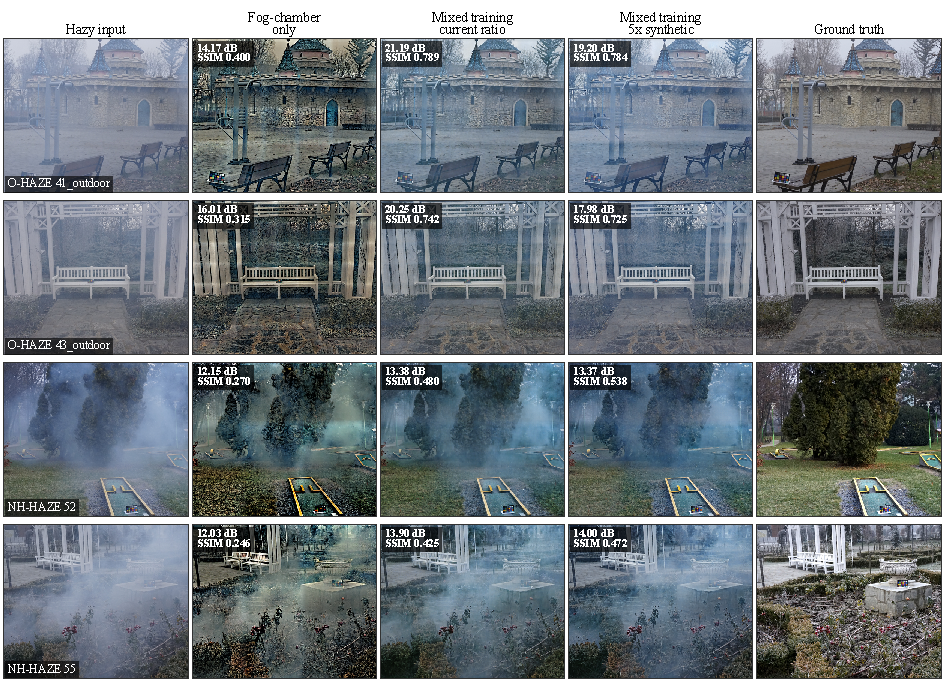
\includegraphics[width=\textwidth]{figures/supplement/figS_mixed_training_ratio_examples.pdf}
\caption{Illustrative public real-haze comparison for four
preselected images (two O-HAZE and two NH-HAZE). The columns show the
hazy input, chamber-only checkpoint, two completed joint-training
schedules, and ground truth. These examples visualize color and overcorrection behavior
and are not a complete-dataset benchmark. The matched mixed schedule
is the primary model; the 5$\times$ model is a sensitivity check.
Because the chamber-only and mixed runs differ in optimization and
training schedule, this is a training-regime comparison rather than
a single-variable ablation.}
\label{figS:mixed_training_examples}
\end{figure}

We also applied the primary mixed-data model without target-domain
training to 99 chamber-free outdoor captures made with a fog machine
placed in front of the camera. Figure~\ref{figS:mixed_free_fog} shows
four preselected examples. Across all 99 captures, mean NIQE changed
from 5.05 for the inputs to 5.54 for the outputs, and NIQE was lower
for 34 of 99 outputs. Because no aligned clear references are available and
NIQE does not measure fog removal, we do not interpret this change as
evidence of improved or degraded restoration. The panel is included
as a qualitative check of applying the mixed model outside the fixed
chamber geometry.

\begin{figure}[htbp]
\centering
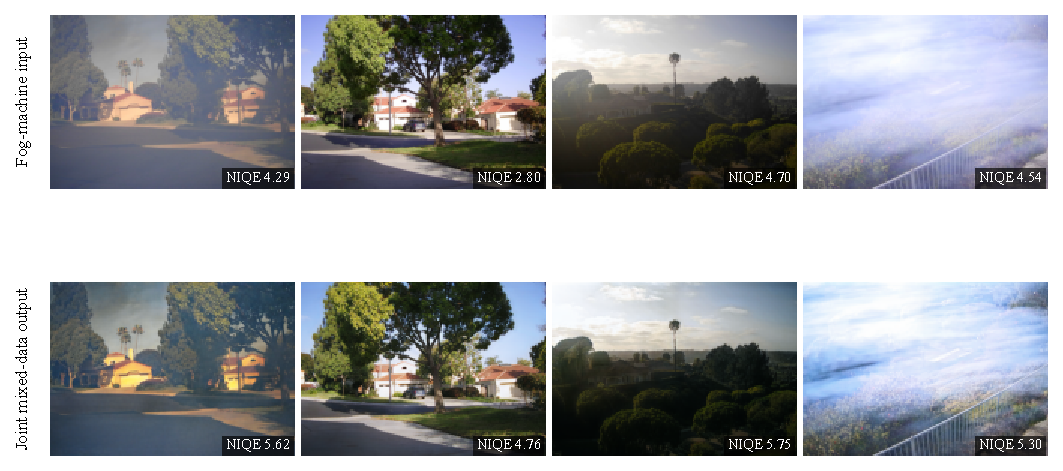
\includegraphics[width=\textwidth]{figures/supplement/figS_mixed_free_fog.pdf}
\caption{Primary joint mixed-data NAFNet applied to four preselected
chamber-free outdoor fog-machine captures (top: input; bottom:
output). The examples show increased contrast together with changes
in color and tone. No aligned clear reference is available. NIQE is
shown per panel as a descriptive natural-image statistic, not as a
fog-removal metric.}
\label{figS:mixed_free_fog}
\end{figure}

\FloatBarrier

\section{Public Paired Real-Haze Adaptation}

The main manuscript reports the combined O-HAZE+NH-HAZE adaptation result. O-HAZE contains 45 paired outdoor real-haze images, and NH-HAZE contains 55 paired non-homogeneous real-haze images~\cite{ancuti2018ohaze,ancuti2020nhhaze}. The reported model used only the combined training policy: O-HAZE images 1--35 and NH-HAZE images 1--45 for training, O-HAZE 36--40 and NH-HAZE 46--50 for validation, and O-HAZE 41--45 plus NH-HAZE 51--55 for testing.

The real-haze fine-tuning run started from the fog-chamber NAFNet model and used random $256 \times 256$ paired hazy/ground-truth crops, L1 reconstruction loss, AdamW, learning rate $10^{-4}$, batch size 4, and early stopping by validation L1. The best validation epoch was 39, and training stopped after epoch 57.

The task-specific result below is intentionally separated from the
mixed model. It tests whether the NAFNet architecture selected by the
chamber benchmark can adapt when paired outdoor haze is available;
it is not used as evidence for zero-shot mixed-model transfer.

\begin{table}[H]
\centering
\scriptsize
\caption{Supervised combined real-haze adaptation protocol and split audit. Image identity was checked as dataset/image-id pairs across train, validation, and test records.}
\label{tabS:external_training_protocol}
\resizebox{\textwidth}{!}{%
\begin{tabular}{@{}>{\raggedright\arraybackslash}p{0.15\textwidth}>{\raggedright\arraybackslash}p{0.27\textwidth}>{\raggedright\arraybackslash}p{0.23\textwidth}>{\raggedright\arraybackslash}p{0.20\textwidth}cc@{}}
\toprule
\textbf{Model} & \textbf{Training images} & \textbf{Validation images} & \textbf{Test images} & \textbf{Best epoch} & \textbf{Overlap} \\
\midrule
Combined real-haze adaptation & O-HAZE 1--35 + NH-HAZE 1--45 (n=80) & O-HAZE 36--40 + NH-HAZE 46--50 (n=10) & O-HAZE 41--45 + NH-HAZE 51--55 (n=10) & 39 & 0 train/test; 0 validation/test \\
\bottomrule
\end{tabular}
}
\end{table}

\begin{table}[H]
\centering
\small
\caption{Internal test-split metrics for the combined real-haze model. Subset rows are diagnostics of the same model.}
\label{tabS:external_heldout}
\begin{tabular}{@{}>{\raggedright\arraybackslash}p{0.20\textwidth}>{\raggedright\arraybackslash}p{0.32\textwidth}cccc@{}}
\toprule
\textbf{Model} & \textbf{Held-out split} & \textbf{n} & \textbf{MAE} & \textbf{PSNR} & \textbf{SSIM} \\
\midrule
Combined real haze & O-HAZE 41--45 & 5 & 0.0589 & 22.65 & 0.726 \\
Combined real haze & NH-HAZE 51--55 & 5 & 0.0894 & 18.77 & 0.640 \\
Combined real haze & O-HAZE 41--45 + NH-HAZE 51--55 & 10 & 0.0741 & 20.71 & 0.683 \\
\bottomrule
\end{tabular}
\end{table}
\FloatBarrier

 

\subsection{NTIRE 2026 Nighttime Haze Evaluation}

The NTIRE 2026 evaluation used the released nighttime haze training pairs. The available training set contains 25 paired nighttime hazy/ground-truth images. We trained an NTIRE-specific NAFNet from the fog-chamber model using IDs 01--20 for training, IDs 21--23 for validation and model selection, and IDs 24--25 as an internal test split. The best validation epoch was 15, and training stopped after epoch 29. This internal split is useful for checking whether the same backbone adapts to nighttime paired haze, but it is not an official challenge validation/test result because those clear targets are unavailable locally. It therefore does not establish a competition rank.

\begin{table}[H]
\centering
\small
\caption{NTIRE 2026 supervised nighttime-haze result. The held-out IDs 24--25 were not used for training or model selection. Metrics are computed against the released training ground truth.}
\label{tabS:ntire26_supervised}
\begin{tabular}{llcccc}
\toprule
\textbf{Split} & \textbf{Model} & \textbf{n} & \textbf{MAE} & \textbf{PSNR} & \textbf{SSIM} \\
\midrule
Held-out 24--25 & NTIRE NAFNet & 2 & 0.0435 & 24.77 & 0.770 \\
\bottomrule
\end{tabular}
\end{table}
\FloatBarrier

The combined real-haze result uses a 10-image internal test split, and the NTIRE 2026 check uses a two-image internal test split from the released training pairs. These checks show that the fog-chamber NAFNet model can be adapted by paired outdoor or nighttime haze supervision, but the training policy, split definition, image size, and reference appearance prevent leaderboard claims.
\FloatBarrier


\section{Fog Density Statistics}

Fog statistics were computed from the 552-image fog-chamber benchmark held-out split and from the clear and light-fog outdoor image sets. Images were converted to numeric pixel values after resizing the longest side to at most 512 pixels for consistent throughput. The dark-channel haze index was the image mean of a 15-pixel minimum-filtered color-channel dark channel, RMS contrast was luminance standard deviation divided by mean luminance, sharpness was the mean finite-difference luminance gradient magnitude, and airlight shift was the change in mean luminance relative to the available clear reference. Chamber statistics used paired fog/clear archive images, so contrast, luminance-standard-deviation, and gradient attenuation were reported as fog-over-clear ratios. The outdoor clear and light-fog captures are independent groups, so outdoor attenuation was reported only as a group-level light-fog/clear ratio.

\begin{figure}[htbp]
\centering

\includegraphics[width=0.95\textwidth]{figures/supplement/figS4_fog_density_proxy_statistics.pdf}
\caption{Simple fog statistics for the chamber and outdoor data. The chamber condition uses paired fog/clear archive references; the outdoor light-fog condition uses the outdoor clear group as an independent reference. Error bars show 95\% confidence intervals for absolute per-image metrics.}
\label{figS:fog_density_proxy}
\end{figure}

\begin{table}[htbp]
\centering
\small
\caption{Fog statistics comparing chamber and outdoor data. Ratios are fog/reference values, where the reference is the paired clear archive image for chamber data and the outdoor clear group mean for outdoor light fog.}
\label{tabS:fog_density_proxy}
\begin{tabular}{lccccc}
\toprule
\textbf{Condition} & \textbf{n} & \textbf{Dark channel} & \textbf{RMS contrast} & \textbf{Grad. mag.} & \textbf{Contrast ratio} \\
\midrule
Benchmark chamber & 552 & 0.526 & 0.142 & 0.00478 & 0.340 \\
Outdoor clear & 430 & 0.211 & 0.639 & 0.02988 & 1.000 \\
Outdoor light fog & 84 & 0.437 & 0.232 & 0.00483 & 0.363 \\
\bottomrule
\end{tabular}
\end{table}

The statistics separated clear and fogged imagery in both acquisition regimes. For the benchmark chamber data, RMS contrast was 0.340 of the paired clear reference and mean gradient was 0.181 of clear. Outdoor light fog also moved in the expected direction relative to outdoor clear: dark-channel haze index increased from 0.211 to 0.437, RMS contrast fell to 0.363 of the clear outdoor group, and mean gradient fell to 0.162 of clear. Thus the statistics support a defensible relative fog-index comparison across chamber and free-space data, but they do not establish physical fog density without distance and calibration.

\section{Image-Domain Power-Spectral Analysis}
\label{secS:psd_image_domain}

We used the paired chamber data to quantify how fog changes spatial-frequency content in the recorded images. For each held-out pair, the foggy chamber capture and the corresponding archive image displayed on the screen were converted to luminance, resized to $512 \times 512$, mean-subtracted, Hann-windowed, Fourier transformed, and radially averaged into 96 spatial-frequency bins. We then computed the per-pair radial power-spectral-density (PSD) ratio,
\begin{equation}
R_{\mathrm{PSD}}(f) =
\frac{P_{\mathrm{fog}}(f)}
     {P_{\mathrm{archive}}(f)} ,
\label{eqS:psd_ratio}
\end{equation}
where $P_{\mathrm{fog}}(f)$ is the foggy camera-capture PSD and $P_{\mathrm{archive}}(f)$ is the PSD of the displayed archive image. The deterministic every-tenth held-out split gave $n=552$ pairs.

This is an image-domain degradation measurement, not a physical transmission spectrum of the fog. The ratio includes the display, chamber, fog, lens, sensor, exposure, camera processing, and resizing pipeline. It is therefore used only to summarize loss of recorded spatial detail.

The median paired PSD ratio was 0.0322 (95\% bootstrap CI 0.0294--0.0372) over low spatial frequencies, 0.01--0.05 cycles/pixel, and 0.0036 (95\% CI 0.0033--0.0041) over higher spatial frequencies, 0.15--0.24 cycles/pixel. Thus high-frequency power was retained 8.9$\times$ less than low-frequency power in the paired image-domain measurement. This frequency-domain result supports the Laplacian-retention analysis in the main text: foggy captures lose fine spatial structure disproportionately, making high-texture scenes harder to restore.

\begin{figure}[htbp]
\centering

\includegraphics[width=0.85\textwidth]{figures/supplement/paired_psd_retention.pdf}
\caption{Paired image-domain power-spectral-density retention for the held-out chamber split. The solid line shows the median foggy-capture/archive PSD ratio across image pairs; the shaded band shows the interquartile range. The dashed line shows the ratio of mean foggy and archive PSDs. Green and orange bands mark the low- and high-frequency ranges summarized in the text.}
\label{figS:paired_psd_retention}
\end{figure}
\FloatBarrier

\section{Paired Structure-Loss Metrics and Restoration Difficulty}
\label{secS:paired_structure_metrics}

We used the 552-image fog-chamber benchmark held-out split to ask whether simple image statistics tracked image-level NAFNet restoration quality. Each foggy image was paired with its aligned clear archive target. We compared foggy-image-only haze proxies with paired structure-loss metrics computed from the fog/clear pair.

The strongest single paired statistic was the mean absolute Laplacian-response ratio,
\begin{equation}
r_{\nabla^2} =
\frac{\mathrm{mean}\left(\left|\nabla^2 I_{\mathrm{fog}}\right|\right)}
{\mathrm{mean}\left(\left|\nabla^2 I_{\mathrm{clear}}\right|\right)} ,
\label{eqS:laplacian_ratio}
\end{equation}
where $I_{\mathrm{fog}}$ and $I_{\mathrm{clear}}$ are luminance images. This ratio measures how much fine spatial structure remains in the foggy image relative to the aligned clear target. It had Spearman correlation $\rho=0.632$ with per-image NAFNet PSNR. By comparison, the strongest foggy-image-only statistic in this subset, the 90th percentile dark-channel response, reached $\rho=0.399$.

We also evaluated the same mean-absolute Laplacian ratio using wider finite-difference steps, where step~1 is the nearest-neighbor five-point Laplacian and larger steps compare pixels separated by 3, 8, or 12 pixels. Correlation with NAFNet PSNR decreased as the step widened ($\rho=0.542$ at step~3 and $0.417$ at step~8), indicating that the most predictive signal was fine-scale structure retention rather than broader luminance variation. A separate PSD fit summarized each fog/clear pair by a single equivalent Gaussian-PSF width, but this scalar blur width was only a weak predictor of restoration quality ($\rho=-0.206$), so we treat it as a diagnostic rather than the primary difficulty metric.

\begin{figure}[htbp]
\centering

\includegraphics[width=\textwidth]{figures/supplement/figS_paired_structure_loss_metric.pdf}
\caption{Paired structure-loss metrics track NAFNet restoration difficulty on the fog-chamber held-out split. (A) Signed Spearman correlations between selected paired and foggy-only image statistics and per-image NAFNet PSNR, with $\rho$ values labeled next to each point. (B) Per-image NAFNet PSNR plotted against the strongest single metric, the scalar fog/clear mean absolute Laplacian-response ratio. Points are colored by archive category, and the black line shows a fit versus $\log_{10}$ of the metric. (C) Example showing the foggy input, aligned clear target, and independently contrast-scaled absolute Laplacian-response maps for clear and foggy images.}
\label{figS:paired_structure_metric}
\end{figure}

The statistic is a scalar ratio of two full-image averages, not the average of a pixelwise ratio map. Thus, locations with larger absolute Laplacian response contribute more to the numerator and denominator, whereas flat regions contribute little. These results suggest that image-level restoration difficulty is not captured by foggy-image haze proxies alone. Paired structure loss, especially loss of Laplacian response, better tracks NAFNet PSNR because it measures how much high-frequency scene detail survives the fog-imaging process. The statistic is a relative restoration-difficulty index, not a calibrated physical fog-density measurement.

\section{Synthetic-Camera and Image-Signal-Processing Sensitivity}
\label{secS:synthetic_camera}

We performed a controlled sensitivity study to separate camera and
image-signal-processing effects from changes in scene content. The study
used 96 images from the held-out fog-chamber split, balanced as 16 images
from each of six archive categories. No model parameters were trained or
selected on these images. Each foggy input $x$ was evaluated under 43
conditions: an unchanged identity condition and 42 nonidentity settings
spanning exposure, white balance, tone response, Gaussian blur, JPEG
compression, sensor shot/read noise, resampling, and combined profiles.
The same deterministic setting and stochastic noise basis were applied to
the foggy input, its aligned clear target, and the baseline model output.

For a fixed model $f$ and camera operator $C$, input-output tracking was
measured from
\begin{equation}
d_{\mathrm{in}}(C)=\mathrm{PSNR}(x,C(x)), \qquad
d_{\mathrm{out}}(C)=\mathrm{PSNR}(f(x),f(C(x))).
\label{eqS:camera_tracking}
\end{equation}
Because larger PSNR indicates a smaller perturbation, a positive
correlation between $d_{\mathrm{in}}$ and $d_{\mathrm{out}}$ indicates
that conditions producing larger input changes tend to produce larger
output changes. Tracking alone does not establish restoration accuracy.
We therefore used unchanged-target accuracy,
\begin{equation}
A_{\mathrm{canonical}}(C)=\mathrm{PSNR}(f(C(x)),y),
\label{eqS:camera_accuracy}
\end{equation}
where $y$ is the aligned clear target, as the primary robustness measure.
Confidence intervals for condition means used image bootstrap resampling;
tracking intervals used 1{,}000 clustered bootstrap resamples that retained
each selected image's complete condition set.

The chamber-trained NAFNet reached 24.000~dB PSNR and
0.7791 SSIM in the identity condition on this 96-image subset, consistent
with its 24.33~dB mean on the complete 552-image benchmark split. Across
the 42 nonidentity condition means, input and output changes were
positively associated (Pearson $r=0.706$, 95\% clustered-bootstrap CI
0.693--0.719; Spearman $\rho=0.665$). The fitted slope was 0.451 (95\%
CI 0.439--0.463), so the curves tracked in ordering but not one-to-one in
decibels. Ordering within individual perturbation families was stronger
($r=0.973$--0.999), showing that severity produced coherent curves even
though response magnitude differed among camera operations.

Camera and processing changes also reduced reconstruction accuracy. The
largest tested failure was the strongest sensor-noise condition, which
reduced canonical-target PSNR by 12.70~dB on average (95\% CI
12.04--13.36~dB loss). Large exposure and white-balance shifts and the
combined profiles also caused substantial losses, whereas the tested
resampling range had little effect. Figure~\ref{figS:synthetic_camera}
combines the tracking analysis with the corresponding
unchanged-target accuracy curves.

\begin{figure}[p]
\centering
\textbf{(a)}\\[-0.2em]

\includegraphics[width=0.92\textwidth]{figures/supplement/figS8_camera_tracking.pdf}
\par\smallskip
\textbf{(b)}\\[-0.2em]

\includegraphics[width=0.92\textwidth]{figures/supplement/figS8_camera_accuracy_curves.pdf}
\caption{Controlled synthetic-camera sensitivity of the fixed
fog-chamber NAFNet checkpoint. (a)~Left: condition-mean input-shift versus output-shift PSNR
for the 42 nonidentity settings; the dashed line denotes equal input and
output change, not a regression fit. Right: mean canonical-target accuracy
change grouped by perturbation family. (b)~Canonical-target accuracy change
as a function of signed setting or normalized severity; shaded bands are
95\% image-bootstrap confidence intervals.}
\label{figS:synthetic_camera}
\end{figure}

These perturbations are controlled abstractions rather than a physical
camera model. They do not reproduce demosaicing, rolling shutter,
autofocus, flare, lens-specific blur, proprietary denoising, high-dynamic-
range fusion, or all interactions among sensor and processing stages.
Consequently, this experiment identifies model sensitivities and supports
the bounded claim that input and output changes track, but it is not a
substitute for paired clear/fog capture using a physically different
camera.
\FloatBarrier

\section*{Supplementary Video Captions}

\textbf{Supplementary Video 1.} Primary joint mixed-data NAFNet
applied framewise to a 16.78-s iPhone~13 aircraft-window video
(left: input; right: output). The model received no target-domain or
temporal training. The video shows the increase in local contrast and
the associated color and tone changes over the complete 1{,}007-frame
sequence. No aligned clear reference is available.

\textbf{Supplementary Video 2.} Primary joint mixed-data NAFNet
applied framewise to a second, foggier 7.43-s iPhone~13
aircraft-window video (left: input; right: output). The complete
446-frame sequence shows stronger contrast together with a persistent
color shift. No aligned clear reference is available, so the video is
a qualitative demonstration rather than a full-reference restoration
test.

\bibliography{defogging_supplement_refs}

\end{document}
